\documentclass[usenames,dvipsnames,handout]{beamer}
% add option handout to collapse frames for handout


% NOTES: https://gist.github.com/andrejbauer/ac361549ac2186be0cdb

\usepackage{amsmath,amssymb,amsfonts}
\usepackage{bibentry}
\usepackage{graphicx}
\usepackage{listings}
\usepackage{inconsolata}
\usepackage[utf8]{inputenc}
\usepackage{multibib}
\usepackage{xcolor}
\usepackage{tikz}
%\usepackage{venndiagram}

\usetikzlibrary{shapes,backgrounds}

% This font supports boldface
\renewcommand{\ttdefault}{pcr}

% % for having fixed columns in escaped text in listings
% \makeatletter
% \let\escapedfixedcolumns\lst@column@fixed
% \makeatother

\newcites{ex}{References}
\newcites{kw}{References for Examples}

\lstdefinelanguage{GF}{
    morekeywords={ abstract, concrete, resource, interface, instance,
        incomplete, of, with, open,
        cat, fun, lincat, lin, oper, flags, param
    },
    escapeinside={(*@}{@*)},
    morecomment=[l]{--},
    morecomment=[s]{\{-}{-\}},
    morestring=[b]",
    commentstyle=\color{OliveGreen}\itshape,
    basicstyle=\footnotesize\ttfamily\bfseries,
    literate={∃}{{$\exists$}}1 {λ}{{$\lambda$}}1 {∧}{{$\land$}}1,
    frame=tbrl,
    rulecolor=\color{gray},
    backgroundcolor=\color{lightgray!30},
}

\lstdefinelanguage{GFcmd}{
    morekeywords={parse, linearize, view_tree},
    morestring=[b]",
    basicstyle=\footnotesize\rmfamily
}

\lstdefinelanguage{XML}{
    basicstyle=\ttfamily\footnotesize,
    morestring=[b]",
    morestring=[s]{>}{<},
    morecomment=[s]{<?}{?>},
    stringstyle=\color{black},
    identifierstyle=\bfseries,
    keywordstyle=\color{cyan},
    %morekeywords={xmlns,version,type}
    showstringspaces=false
}

\newcommand{\gfcmd}[1]{\lstinline[language=GFcmd]{#1}}
\newcommand{\gfinl}[1]{\lstinline[language=GF]{#1}}
\def\str#1{\emph{``#1''}}   % Examples in natural language
\def\strf#1{``\emph{#1}''}   % Examples as formula
\def\log#1{{\bfseries#1}}              % Examples in logical representation
\def\strcol#1{\textcolor{NavyBlue}{#1}}
\def\strcoll#1{\textcolor{Red}{#1}}

\title{High-Precision Semantics Extraction for Mathematics}
\author{Jan Frederik Schaefer}
\institute{GF Summer School 2018 \\ Stellenbosch, South Africa}
\date{\today} 

% \usetheme{Madrid}
\usetheme{Pittsburgh}
\setbeamertemplate{footline}[frame number]
\setbeamertemplate{navigation symbols}{}
\usecolortheme{beaver}

\begin{document}
\bibliographystyleex{acm}
\bibliographystylekw{alpha}


% following lines for slide numbers
\expandafter\def\expandafter\insertshorttitle\expandafter{%
  \insertshorttitle\hfill%
  \insertframenumber\,/\,\inserttotalframenumber}

\frame{\titlepage}


\frame{
    \frametitle{\texttt{whoami}}
    \begin{itemize}
        \item MSc Student, Computer Science
        \item FAU (\textbf{F}riedrich-\textbf{A}lexander-\textbf{U}niversit\"at Erlangen-N\"urnberg) \\ (in Southern Germany)
        \item KWARC research group
            \begin{itemize}
                \item Led by Michael Kohlhase
                \item Knowledge representation and reasoning techniques
                \item Focus on mathematical content
            \end{itemize}
    \end{itemize}
}

\frame{
    \frametitle{Motivation: SMGloM}
    \begin{itemize}
        \item A \emph{\textbf{S}emantic, \textbf{M}ultilingual \textbf{Glo}ssary of \textbf{M}athematics}
        \item Definitions of mathematical terms
        \item Semantic information about dependencies
    \end{itemize}

    \vspace{1.5em}
    1714 words defined, the language coverage is:

    \vspace{1em}
    \begin{tabular}{l | r}
        English & $94.0\%$ \\
        German & $69.8\%$ \\
        Chinese (simplified) & $8.5\%$ \\
        Romanian & $3.5\%$ \\
        \ldots & \\
        Afrikaans & $0.0\%$ \\
    \end{tabular}

    \vspace{1.5em}
    \emph{\ldots let's use GF!}
}

\frame{
    \frametitle{Motivation: SMGloM}
    
    Example adapted from \citekw{GinIanJuc:spsttom16}:
    \vspace{0.5em}

    \str{A non-empty \strcol{graph} $G$ is said to be \textbf{connected}, if
    any two of its \strcol{nodes} are linked by a \strcol{path} in $G$.}

    \vspace{1em}

    \str{Ein nicht-leerer \strcol{Graph} $G$ hei{\ss}t \textbf{zusammenh\"angend}, wenn 
    je zwei seiner \strcol{Knoten} durch einen \strcol{Weg} in $G$ verbunden sind.}
    % \str{Ein \strcol{Graph} $G$ hei{\ss}t \textbf{zusammenh\"angend}, wenn 
    % je zwei seiner \strcol{Knoten} durch einen \strcol{Weg} verbunden sind.}
}


\frame{
    \frametitle{Example}
    \centering
    \str{An integer $n$ is called even iff $2 | n$.}

    \vspace{1em}$\Downarrow$ \gfcmd{parse}

    \vspace{1em}\includegraphics[width=0.8\textwidth]{figures/even-def-tree.png} 

    \vspace{1em}$\Downarrow$ \gfcmd{linearize}

    \vspace{1em}\str{Eine ganze Zahl $n$ hei{\ss}t gerade genau dann, wenn $2 | n$.}
}


\frame{
    \frametitle{We want more...}
    \begin{itemize}
        \item Let's try to formalize sentences
        \item Example: \log{$\forall n . \text{int} ( n ) \Rightarrow ( \text{even} ( n ) \Leftrightarrow \text{divides} ( 2 , n ) )$}
        \item I will present two different approaches
    \end{itemize}
}


\frame{
    \frametitle{First Approach}
    The formal representation is just another language:
    \vspace{2em}

    \includegraphics[width=0.8\textwidth]{figures/project-overview-2.png} 
}

\frame{
    \frametitle{First Approach - Example}
    \centering
    \str{An integer $n$ is called even iff $2 | n$.}

    \vspace{1em}$\Downarrow$ \gfcmd{parse}

    \vspace{1em}\includegraphics[width=0.4\textwidth]{figures/even-def-tree.png} 

    \vspace{1em}$\Downarrow$ \gfcmd{linearize}

    \vspace{1em}\log{$( \forall n . ( ( \lambda x. \text{int} ( x ) ) n ) \Rightarrow ( ( \lambda x. \text{even} ( x ) ) n \Leftrightarrow \text{divides} ( 2 , n ) ) )$}

    \vspace{1em}$\Downarrow$ external simplifier

    \vspace{1em}\log{$\forall n. \text{int}(n) \Rightarrow ( \text{even}(n) \Leftrightarrow \text{divides}(2, n))$}
}

\frame{
    \frametitle{Second Approach}
    Use an external system (MMT) for the logic:
    \vspace{2em}

    \includegraphics[width=\textwidth]{figures/project-overview-3.png}
}


\frame{
    \frametitle{For now: First Approach}

    \includegraphics[width=\textwidth]{figures/project-overview-2-2.png} 
}



\frame{
    \frametitle{Mathematical Language - $\exists$ Formulas}
    There are formulas in the text:
    \vspace{1em}

    \str{A sequence \strcol{$x = \{x_n\}_{n=1}^\infty \in l^\infty(V)$} is called quasi-almost convergent to \strcol{$v \in V$} if \strcol{$\forall L \in \Pi$}, \strcol{$L(x-\widetilde{v}) = 0$}.} \citeex{0906.4010}
    % \str{For any \strcol{graph} $G$, $\alpha_1(G) \le \frac{nb(G)}{4}$.} \citeex{1311.5332}

    \vspace{2em}

    \pause

    There is text in the formulas:
    \vspace{1em}

    % \strf{$L := \{x\in S : \text{$x\in A_i$ \strcol{for all except finitely many} $i$}\}$}
    \strf{$H(P) = \{\text{$\alpha \in \mathbb{N}_0$} ~| ~\text{\strcol{there exists a rational function $f$ on $C$ }} \linebreak[1] \text{\strcol{with $(f)_\infty = \alpha P$}}\}$} \citeex{1311.4143}
}


\frame{
    \frametitle{Grammar Architecture}
    \centering
    \includegraphics[width=0.9\textwidth]{figures/grammar-dichotomy.png}
    \vspace{1em}

    \begin{columns}
        \begin{column}{0.5\textwidth}
            \centering
            Depends on language
        \end{column}
        \begin{column}{0.5\textwidth}
            \centering
            Depends on representation
        \end{column}
    \end{columns}
}


\begin{frame}[fragile]
    \frametitle{There is No Standard Formula Representation}
%     Example: $x^2+1$
%     \vspace{1em}
% 
%     \LaTeX{} representation: \lstinline[basicstyle=\ttfamily]{$x^2+1$}
%     \vspace{1em}

    %% Careful: AsciiMath is particular standard
%%    ASCII representation: \lstinline[basicstyle=\ttfamily]{x^2 + 1}
%%    \vspace{1em}

    \textbf{Example:}

    \vspace{0.5em}
    \str{\strcol{$x^2 + 1$} is greater than or equal to \strcol{$\sqrt{x^2 + 1}$}.}

    \pause
    \vspace{2em}
    \textbf{First Idea:}

    \vspace{0.5em}
    {\footnotesize \textbf{\texttt{\strcol{x{\textasciicircum}2 + 1} is greater than or equal to \strcol{SQRT(x{\textasciicircum}2 + 1)}.}}}

    \pause
    \vspace{2em}
    \textbf{LaTeX:}

    \vspace{0.5em}
    {\footnotesize \textbf{\texttt{\strcol{\$x{\textasciicircum}2 + 1\$} is greater than or equal to \strcol{\${\textbackslash}sqrt\{x{\textasciicircum}2 + 1\}\$}.}}}
\end{frame}


\begin{frame}[fragile]
    \frametitle{Formula Representations - MathML}
    Formula: $x^2 + 1$
    
    \vspace{2em}
    \begin{columns}[T]
        \begin{column}{0.4\textwidth}
            Presentation MathML
            \begin{lstlisting}[language=XML]
<math>
    <mrow>
        <msup>
            <mi>x</mi>
            <mn>2</mn>
        </msup>
        <mo>+</mo>
        <mn>1</mn>
    </mrow>
</math>
\end{lstlisting}
        \end{column}
        \begin{column}{0.4\textwidth}
            Content MathML
            \begin{lstlisting}[language=XML]
<math>
  <apply>
    <plus />
    <apply>
      <power />
      <ci>x</ci>
      <cn>2</cn>
    </apply>
    <cn>1</cn>
  </apply>
</math>
\end{lstlisting}

        \end{column}
    \end{columns}

    \pause
    \vspace{2em}
    %\LaTeX $\;\to$ MathML through \texttt{LaTeXML} \citekw{Miller:latexml:base}
    $$ \text{\LaTeX} \quad \stackrel{\text{LaTeXML}}{\xrightarrow{\hspace*{2cm}}} \quad \text{MathML}\quad\quad\quad\text{(see  \citekw{Miller:latexml:base})}$$
\end{frame}

%% COPY
\frame{
    \frametitle{Remember: Grammar Architecture}
    \centering \includegraphics[width=0.9\textwidth]{figures/grammar-dichotomy.png} \vspace{1em}

    \begin{columns}
        \begin{column}{0.5\textwidth} \centering Depends on language \end{column}
        \begin{column}{0.5\textwidth} \centering Depends on representation \end{column}
    \end{columns}
}


%% TODO: Reference weak type theory

\frame{
    \frametitle{Mathematical Language - Sentence Level}
    \textbf{Definitions:}

    \vspace{0.5em}
    \str{An integer $n$ is called \textbf{even} iff $2 | n$.}

    \vspace{2em}
    \textbf{Declarations:}

    \vspace{0.5em}
    \str{Let $\widetilde{H}$ be a numerical semigroup.} \citeex{1311.4143}

    \vspace{2em}
    \textbf{Statements:}

    \vspace{0.5em}
    \str{For any graph $G$, $\alpha_1(G) \le \frac{nb(G)}{4}$.} \citeex{1311.5332}
}

\frame{
    \frametitle{Mathematical Language - Phrase Level}
    \textbf{Mathematical Objects:}

    \vspace{0.5em}
    \str{An \strcol{integer} $n$ is called \textbf{even} iff $2 | n$.}

    \vspace{0.5em}
    \str{Let $\widetilde{H}$ be a \strcol{numerical semigroup}.} \citeex{1311.4143}

    \vspace{0.5em}
    \str{For any \strcol{graph} $G$, $\alpha_1(G) \le \frac{nb(G)}{4}$.} \citeex{1311.5332}

    \vspace{2em}
    \textbf{Mathematical Properties:}

    \vspace{0.5em}
    \str{An integer $n$ is called \strcol{\textbf{even}} iff $2 | n$.}

    \vspace{0.5em}
    \str{If $x = \{x_n\}_{n=1}^\infty \in l^\infty(V)$ is \strcol{strongly almost convergent in $V$}, then [...]} \citeex{0906.4010}
}


%% COPY
\frame{
    \frametitle{Remember: Grammar Architecture}
    \centering \includegraphics[width=0.9\textwidth]{figures/grammar-dichotomy.png} \vspace{1em}

    \begin{columns}
        \begin{column}{0.5\textwidth} \centering Depends on language \end{column}
        \begin{column}{0.5\textwidth} \centering Depends on representation \end{column}
    \end{columns}
}

\frame{
    \frametitle{Mathematical Language - Formula Level}
    \textbf{Formula Statement:}

    \vspace{0.5em}
    \str{An integer $n$ is called \textbf{even} iff \strcol{$2 | n$}.}

    \vspace{0.5em}
    \str{Since \strcol{$uv \notin A$}, this implies that \strcol{$uz \in A$} and \strcol{$vz \in A$}} \citeex{1311.5332}
    % \str{For any graph $G$, \strcol{$\alpha_1(G) \le \frac{nb(G)}{4}$}.} \citeex{1311.5332}

    \vspace{2em}
    \textbf{Objects:}
    
    \vspace{0.5em}
    \str{\,\strcol{$\bigcup_{i\in I} O_i$} is open in \strcol{$Y$}.}

    \vspace{0.5em}
    \str{The stabilizer in \strcol{$G^\mathbb{C}$} for \strcol{$p$} is an algebraic group.} \citeex{1311.2873}

    \vspace{2em}
    \textbf{(Restricted) Identifier:}

    \vspace{0.5em}
    \str{An integer \strcol{$n$} is called \textbf{even} iff $2 | n$.}

    \vspace{0.5em}
    \str{Let \strcol{$r \ge 2$} be an integer.}
}

\frame{
    \frametitle{Mathematical Language - Formula Atoms}
    \textbf{Numerals:} $2$, $19$, \ldots

    \vspace{2em}
    \textbf{Identifiers:} $n$, $\varphi$, $G$, \ldots

    \vspace{2em}
    \textbf{Binary Operators:} $+$, $\cap$, \ldots

    \vspace{2em}
    \textbf{Binary Relations:} $\ge$, $\in$, \ldots

    \vspace{2em}
    Example: $n^2 + 19 \ge n^2$

    \vspace{2em}
    See also \citekw{Ginev-11}
}

\begin{frame}[fragile]
    \frametitle{Parsing a Formula - Binary Relations}
    Example: \strf{$n > 1$}

    \begin{lstlisting}[language=GF]
-- abstract grammar:
greater_than : FExpression -> FExpression -> FStatement;

-- concrete grammar:
greater_than a b = a ++ ">" ++ b;
    \end{lstlisting}

    \vspace{0.5em}

    \pause
    Better way:
    \begin{lstlisting}[language=GF]
-- abstract grammar:
apply_bin_rel : FBinRelation -> FExpression ->
        FExpression -> FStatement;

-- concrete grammar could be:
apply_bin_rel rel a b = a ++ rel ++ b;
    \end{lstlisting}
\end{frame}

\begin{frame}[fragile]
    \frametitle{Parsing a Formula - Binary Relations}
    The first solution couldn't handle the following cases nicely:
    \begin{itemize}
        \item \strf{$1 < m < n$}
        \item \strf{$0 \le r < 1$}
        \item \strf{$0 = t_0 < t_1 < \ldots < t_n = 1$}
    \end{itemize}
    
    \vspace{1.5em}

    \pause
    Cases like \strf{$0 \le r < 1$} are easy with better approach:
    \begin{lstlisting}[language=GF]
-- abstract grammar:
apply_tern_rel : FBinRelation -> FBinRelation->
        FExpression -> FExpression -> FExpresion ->
        FStatement;
    \end{lstlisting}
    \begin{lstlisting}[language=GF]
-- concrete grammar:
apply_tern_rel rel1 rel2 a b c = a ++ rel1 ++ b ++
                                      rel2 ++ c;
    \end{lstlisting}
\end{frame}

% \frame{
%     \frametitle{Grammatical Roles of Formulas}
%     Clauses:
%     \begin{itemize}
%         \item \str{Further observe that \strcol{$|V(H)| \le 2m$}} \citeex{1311.5471}
%         \item \str{Since \strcol{$uv \notin A$}, this implies that \strcol{$uz \in A$} and \strcol{$vz \in A$}} \citeex{1311.5332}
%     \end{itemize}
%     \vspace{0.5em}
% 
%     Noun phrases:
%     \begin{itemize}
%         \item \str{The stabilizer in \strcol{$G^\mathbb{C}$} for \strcol{$p$} is an algebraic group.} \citeex{1311.2873}
%     \end{itemize}
%     \vspace{0.5em}
% 
%     Numbers:
%     \begin{itemize}
%         \item \str{Hence $G[N_A(u)\cup N_A(v)]$ is bipartite with \strcol{$d_A(u) + d_A(v)$} vertices.} \citeex{1311.5332}
%     \end{itemize}
%     \vspace{0.5em}
% 
%     Less clear examples:
%     \begin{itemize}
%         \item \str{an \strcol{$n$}-dimensional vector space}
%         \item \str{if \strcol{$n \in S$} is even\ldots}
%         \item \str{there is an integer \strcol{$n > 2$} such that\ldots}
%     \end{itemize}
% }

%% COPY
\frame{
    \frametitle{Recall: Mathematical Language - Formula Level}
    \textbf{Formula Statement:}

    \vspace{0.5em}
    \str{An integer $n$ is called \textbf{even} iff \strcol{$2 | n$}.}

    \vspace{0.5em}
    \str{Since \strcol{$uv \notin A$}, this implies that \strcol{$uz \in A$} and \strcol{$vz \in A$}} \citeex{1311.5332}
    % \str{For any graph $G$, \strcol{$\alpha_1(G) \le \frac{nb(G)}{4}$}.} \citeex{1311.5332}

    \vspace{2em}
    \textbf{Objects:}
    
    \vspace{0.5em}
    \str{\,\strcol{$\bigcup_{i\in I} O_i$} is open in \strcol{$Y$}.}

    \vspace{0.5em}
    \str{The stabilizer in \strcol{$G^\mathbb{C}$} for \strcol{$p$} is an algebraic group.} \citeex{1311.2873}

    \vspace{2em}
    \textbf{(Restricted) Identifier:}

    \vspace{0.5em}
    \str{An integer \strcol{$n$} is called \textbf{even} iff $2 | n$.}

    \vspace{0.5em}
    \str{Let \strcol{$r \ge 2$} be an integer.}
}

\frame{
    \frametitle{Example: \strf{$n > 2$} as Statement}
    \str{we know that \strcol{$n > 2$}}

    \includegraphics[width=0.6\textwidth]{figures/ng2_stmt.png}

    In logic: \log{$\text{greater}(n, 2)$}
}

\begin{frame}
    \frametitle{Example: \strf{$n > 2$} as Identifier}
    \str{there is an integer \strcol{$n > 2$} such that\ldots}

    \includegraphics[width=0.6\textwidth]{figures/ng2_id.png}

    \log{$(\exists \strcoll{n}.(\lambda x.\text{int}(x))\strcoll{n} \land \text{\strcol{greater$(n, 2)$}} \land (\ldots))$}

    \vspace{1em}$\Downarrow$ external simplifier

    \vspace{1em}\log{$\exists \strcoll{n}.\text{int}(\strcoll{n}) \land \text{\strcol{greater$(n, 2)$}} \land \ldots$}
\end{frame}

\begin{frame}[fragile]
    \frametitle{Example: \strf{$n > 2$} as Identifier}
    We need to extract \strf{$n$} from \strf{$n > 2$}:

    \begin{lstlisting}[language=GF]
-- Identifier record (simplified)
Identifier = {
    formula : Str;  -- the restriction, e.g. greater(n, 2)
    (*@\strcol{core : Str}@*);    -- the identifier, e.g. n
};
    \end{lstlisting}
    \pause
    \begin{lstlisting}[language=GF]
-- example usage
fcid_fbinrel_fexpr_to_identifier a r1 b = {
    formula = r1 ++ "(" ++ a ++ "," ++ b ++ ")";
    (*@\strcol{core = a;}@*)
};
    \end{lstlisting}
    \begin{lstlisting}[language=GF]
-- for statements like (∃n.(λx.int(x))n ∧ greater(n,2))
exists_statement obj id = inp("∃" ++ (*@\strcol{id.core}@*) ++ "."
        ++ lwrap(obj) ++ (*@\strcol{id.core}@*) ++ (*@\strcol{and\_formula(id)}@*));
    \end{lstlisting}
\end{frame}


\frame{
    \frametitle{Mathematical Objects (\gfinl{MObj})}

    Examples:
    \begin{itemize}
        \item \str{\strcol{integer}}
        \item \str{an \strcol{even integer}}
        \item \str{There is a \strcol{bijective map from $(0,1)$ to $\mathbb{R}$}}
        \item \str{There is a \strcol{bijective map} \strcoll{$f$} \strcol{from $(0,1)$ to $\mathbb{R}$}}
        \item \str{Let $C$ be a \strcol{complete nonsingular irreducible curve over an algebraically closed field $k$ of characteristic 0}} \citeex{1311.4143}
    \end{itemize}
    
}

\begin{frame}[fragile]
    \frametitle{Mathematical Objects (\gfinl{MObj})}
    \begin{lstlisting}[language=GF]
exists_suchthat :
    PosNegPol           -- is/isn't
    -> MObj             -- integer
    -> Identifier       -- n
    -> StatementFin     -- ...
    -> StatementFin;
    \end{lstlisting}

    \vspace{1em}
    \str{there is an \strcol{integer} $n$ such that \ldots}

    \vspace{1em}
    \log{$\exists n . \strcol{\text{int}} ( n ) \land \ldots$}
\end{frame}

\begin{frame}[fragile]
    \frametitle{Mathematical Objects (\gfinl{MObj})}
    \begin{lstlisting}[language=GF]
exists_suchthat :
    PosNegPol           -- is/isn't
    -> MObj             -- positive even integer
    -> Identifier       -- n
    -> StatementFin     -- ...
    -> StatementFin;
    \end{lstlisting}

    \vspace{1em}
    \str{there is a \strcol{positive even integer} $n$ such that \ldots}

    \vspace{1em}
    \log{$\exists n . \strcol{\text{pos}} ( n ) \land \strcol{\text{even}} ( n ) \land \strcol{\text{int}} ( n ) \land \ldots$}

    \pause
    \vspace{1em}
    \log{$\exists n . \strcol{(\lambda x.\text{pos}(x) \land \text{even}(x) \land \text{int}(x) )} n \land \ldots$}
\end{frame}


\frame{
    \frametitle{Intersective Interpretation of Adjectives}

    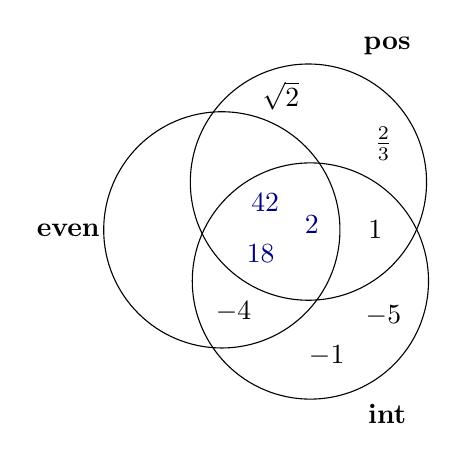
\begin{tikzpicture}
        \draw (60:0.7cm) circle (1.5cm); % node[below] {\log{\text{pos}}};
        \draw (180:0.75cm) circle (1.5cm); % node[below] {\log{\text{even}}};
        \draw (300:0.75cm) circle (1.5cm); % node[below] {\log{\text{int}}};
        % \draw node at (60:1.55cm) {\log{\text{pos}}};
        % \draw node at (180:1.55cm) {\log{\text{even}}};
        % \draw node at (300:1.55cm) {\log{\text{int}}};
        \draw node at (60:2.7cm) {\log{\text{pos}}};
        \draw node at (180:2.7cm) {\log{\text{even}}};
        \draw node at (300:2.7cm) {\log{\text{int}}};

        \draw node at (90:1.7cm) {$\sqrt{2}$};
        \draw node at (40:1.7cm) {$\frac{2}{3}$};
        \draw node at (320:1.7cm) {$-5$};
        \draw node at (290:1.7cm) {$-1$};

        \draw node at (240:1.2cm) {$-4$};
        \draw node at (0:1.2cm) {$1$};

        \draw node at (10:0.4cm) {$\strcol{2}$};
        \draw node at (120:0.4cm) {$\strcol{42}$};
        \draw node at (230:0.4cm) {$\strcol{18}$};
    \end{tikzpicture}

    \begin{itemize}
        \item \str{Positive even integers} are the intersection of integers, even things and positive things
        \item This doesn't work for every adjective!
    \end{itemize}

    % \begin{venndiagram3sets}[labelA=\log{\text{pos}}, labelB=\log{\text{even}}, labelC=\log{\text{int}}, shade=lightgray!30]
    % \fillACapBCapC
    % \setpostvennhook
    % {
    %     \draw (labelA) ++(250:8ex) node{$\sqrt{2}$};
    %     \draw (labelA) ++(300:3ex) node{$\frac{2}{3}$};
    % }
    % \end{venndiagram3sets}
}

\frame{
    \frametitle{Definitions}
    \str{An integer $n$ is called even iff $2 | n$.}

    \vspace{1em}

    Idea: \log{$\text{even}(n) \Leftrightarrow \text{divides}(2, n)$}

    \pause
    \vspace{1em}
    With quantifier: \log{$\forall n. \text{int}(n) \Rightarrow ( \text{even}(n) \Leftrightarrow \text{divides}(2, n))$}

    \vspace{1em}
    What's generated: \log{$( \forall n . ( ( \lambda x. \text{int} ( x ) ) n ) \Rightarrow ( ( \lambda x. \text{even} ( x ) ) n \Leftrightarrow \text{divides} ( 2 , n ) ) )$}
}

\frame{
    \frametitle{A Bigger Example}

    \str{A positive integer $n$ is called prime, iff there is no integer $1 < m < n$ such that $m | n$}

    \vspace{1em}
    \textbf{Translation to (from) German:}
    \vspace{0.2em}

    \str{Eine positive ganze Zahl $n$ ist prim genau dann, wenn es keine ganze Zahl $1 < m < n$ gibt, sodass $m | n$}

    \vspace{1em}
    \textbf{Formalization:}
    \vspace{0.2em}

    \log{$( \forall n . ( ( \lambda x. \text{pos} ( x ) \land \text{int} ( x ) ) n ) \Rightarrow ( ( \lambda x. \text{prime} ( x ) ) n \Leftrightarrow ( \lnot \exists m . ( \lambda x. \text{int} ( x ) ) m \land \text{less} ( 1 , m ) \land \text{less} ( m , n ) \land ( \text{divides} ( m , n ) ) ) ) )$}

    \vspace{1em}$\Downarrow$ external simplifier

    \vspace{1em}\log{$\forall n . \text{pos} ( n ) \land \text{int} ( n ) \Rightarrow ( \text{prime} ( n ) \Leftrightarrow \lnot \exists m . \text{int} ( m ) \land \text{divides} ( m , n ) \land \text{less} ( 1 , m ) \land \text{less} ( m , n ) )$}
}


\frame{
    \frametitle{First Approach - Summary}

    \centering\includegraphics[width=0.7\textwidth]{figures/project-overview-2-2.png} 

    \vspace{2em}

    \begin{itemize}
        \item \textbf{\texttt{+}} Parsing and logic generation in one tool (GF)
        \item \textbf{\texttt{-}} Grammar engineering gets complicated
        \item \textbf{\texttt{-}} We need an external tool for simplification and reasoning
    \end{itemize}
}


\frame{
    \frametitle{Second Approach: Semantics Modelling in MMT}

    \centering\includegraphics[width=0.8\textwidth]{figures/project-overview-3.png} 
}


\frame{
    \frametitle{What is MMT?}
    \begin{itemize}
        \item \emph{Meta Meta Tool}
        \item Foundation-independent
        \item A lot of features for mathematical knowledge management
        \item See e.g. \citekw{Rabe:mmtsys:16}
        \item We'll focus only on a small ``slice'' of MMT
    \end{itemize}
}

\begin{frame}[fragile]
    \frametitle{Types for \texttt{\bfseries cat}s}
    \includegraphics[scale=0.4]{figures/mobjparse.png}

    \vspace{1.2em}
    \log{$\lambda x.\text{pos}(x) \land \text{even}(x) \land \text{int}(x)$}
\end{frame}

\begin{frame}[fragile]
    \frametitle{Types for \texttt{\bfseries cat}s}
    \log{$\lambda x.\text{pos}(x) \land \text{even}(x) \land \text{int}(x)$}

    \vspace{1.0em}
    Type declarations for atoms:

    \vspace{0.5em}
    \quad\includegraphics[scale=0.2]{figures/naive_type_decls.png}

    \pause
    \vspace{2.0em}
    \emph{Better:} Types for \texttt{\bfseries cat}s in MMT:

    \vspace{0.5em}
    \quad\includegraphics[scale=0.2]{figures/cat_types_example.png}

    \vspace{0.5em}
    \quad\includegraphics[scale=0.2]{figures/cat_types_example_pt2.png}

\end{frame}


\begin{frame}[fragile]
    \frametitle{Grammar Nodes: \texttt{\bfseries restrict\char`_mobj } }

    \includegraphics[scale=0.4]{figures/restrict_graph.png}

    \vspace{1.5em}
    Goal: $\text{\bfseries restrict even integer} = \lambda x.\text{\bfseries even}(x) \land \text{\bfseries integer}(x)$

    \pause
    \vspace{1.0em}
    \quad\includegraphics[scale=0.2]{figures/restrict_mmt_def.png}

    \pause
    \vspace{2em}
    We can map the GF tree to an MMT term:

    \vspace{0.5em}
    \gfinl{restrict_mobj even_MObjProp integer_MObj}

    \vspace{0.2em}
    \quad$\Downarrow$ {\tiny GF-MMT-Bridge}
    
    \vspace{0.2em}
    \includegraphics[scale=0.2]{figures/even_int_mmt.png}
\end{frame}

\begin{frame}[fragile]
    \frametitle{MMT Theories}

    \begin{columns}
        \begin{column}{0.45\textwidth}
            \lstinputlisting[language=GF,basicstyle=\scriptsize\ttfamily\bfseries]{gf/Cats.gf}

            \lstinputlisting[language=GF,basicstyle=\scriptsize\ttfamily\bfseries]{gf/Lexicon.gf}

            \lstinputlisting[language=GF,basicstyle=\scriptsize\ttfamily\bfseries]{gf/Grammar.gf}
        \end{column}

        \begin{column}{0.45\textwidth}
            \includegraphics[scale=0.2]{figures/cats_mmt.png}

            \vspace{0.8em}
            \includegraphics[scale=0.2]{figures/lexicon_mmt.png}

            \vspace{0.8em}
            \includegraphics[scale=0.2]{figures/grammar_mmt.png}
        \end{column}
    \end{columns}
\end{frame}

\frame{
    \frametitle{Framework for Language Semantics Experiments}

    \begin{minipage}{\textwidth}
        \centering\includegraphics[width=0.6\textwidth]{figures/project-overview-3.png} 
    \end{minipage}

    \vspace{2.5em}

    \setlength{\arrayrulewidth}{1.0pt}
    \quad\quad\begin{tabular}{r@{\hskip3pt} l l}
        \vspace{0.1em}&\strcol{GF} &\textit{(= \strcol{grammar} development framework)}\\
        \vspace{0.1em}+&\strcol{MMT} &\textit{(= \strcol{logic} development framework)}\\
        \hline
        \\[-1em]
        &\strcol{???} &\textit{(= \strcol{semantics} development framework)}\\
    \end{tabular}
}


\frame{
    \frametitle{Defining a Logic in MMT}
    \includegraphics[scale=0.2]{figures/cats_mmt.png}

    \vspace{2em}
    $\to$ Where does FOL come from?

    \pause
    \vspace{2em} 
    \includegraphics[scale=0.2]{figures/theory_FOL.png}
}

\frame{
    \frametitle{Defining a Logic in MMT}

    \includegraphics[scale=0.2]{figures/theory_PL.png}
}

%% COPY
\frame{
    \frametitle{Framework for Language Semantics Experiments}

    \begin{minipage}{\textwidth}
        \centering\includegraphics[width=0.6\textwidth]{figures/project-overview-3.png} 
    \end{minipage}

    \vspace{2.5em}

    \setlength{\arrayrulewidth}{1.0pt}
    \quad\quad\begin{tabular}{r@{\hskip3pt} l l}
        \vspace{0.1em}&\strcol{GF} &\textit{(= \strcol{grammar} development framework)}\\
        \vspace{0.1em}+&\strcol{MMT} &\textit{(= \strcol{logic} development framework)}\\
        \hline
        \\[-1em]
        &\strcol{???} &\textit{(= \strcol{semantics} development framework)}\\
    \end{tabular}
}

\frame{
    \frametitle{Application: Teaching NL Semantics}
    We use this already in class:

    Students
    \begin{itemize}
        \item write small GF grammars
        \item write the required logic in MMT
        \item define the semantics using that logic
        \item write small theorem provers etc. for inference on natural language input
    \end{itemize}
}

\frame{
    \frametitle{Application: Correctness Checking}

    Very hard!!

    \vspace{2em}
    See also \citekw{Zinn:MathematicalDiscourse} and \citekw{Wolska:PHD}.
}

\frame{
    \frametitle{Better Translations}

    \str{From $A \,\strcol{\subset}\, B$ and $B \,\strcol{\subset}\, A$ it follows that $A = B$.}
    \vspace{1.0em}
    
    \strf{$\strcol{\subset}$} might refer to \strf{$\subseteq$} or to \strf{$\subsetneq$}

    \vspace{1.0em}
    $\to$ we get at least $2 \cdot 2 = 4$ parse trees

    \vspace{1.0em}
    $\to$ we can discard some of them:
    
    \vspace{1.0em}
    \quad Example: Interpreting both \strf{$\strcol{\subset}$} as \strf{$\subsetneq$}:

    \vspace{0.5em}
    \quad\log{$(\subseteq(A, B) \land A \,\strcoll{\ne}\, B) \land (\subseteq(B, A) \land A \,\strcoll{\ne}\, B),\;\;A \,\strcoll{=}\, B$}
}

\frame{
    \frametitle{Knowledge Formalization}
    
    \str{an integer $n$ is called even iff $2|n$}

    \vspace{2.0em}
    \quad\includegraphics[scale=0.2]{figures/even_formalization_mmt_2.png}
}

\frame{
    \frametitle{Summary}

    \begin{itemize}
        \item Math Linguistics/Translation
        \item Semantics Development Framework:
    \end{itemize}

    \setlength{\arrayrulewidth}{1.0pt}
    \quad\quad\begin{tabular}{r@{\hskip3pt} l l}
        \vspace{0.1em}&\strcol{GF} &\textit{(= \strcol{grammar} development framework)}\\
        \vspace{0.1em}+&\strcol{MMT} &\textit{(= \strcol{logic} development framework)}\\
        \hline
        \\[-1em]
        &\strcol{???} &\textit{(= \strcol{semantics} development framework)}\\
    \end{tabular}

    \pause
    \vspace{2.0em}
    \begin{tabular}{r l}
    \textbf{\emph{Advertisement:}}
        &\textbf{SIGMathLing}\\
        &\textbf{S}pecial \textbf{I}nterest \textbf{G}roup on \textbf{Math}s \textbf{Ling}uistics\\
        &\textit{\href{https://sigmathling.kwarc.info/}{https://sigmathling.kwarc.info/}}\\
    \end{tabular}

    \begin{itemize}
        \item \emph{arXMLiv} corpus: 1,232,186 HTML5 scientific documents from the arXiv.org
        \item \emph{GloVe} word embeddings for mathematics
        \item \ldots
    \end{itemize}
}

\frame{
    \frametitle{Bonus: PL Semantics in MMT}

    \includegraphics[scale=0.2]{figures/plsemantics.png}
}

\frame{
    \frametitle{Bonus: Modular Math in MMT}

    \includegraphics[width=\textwidth]{figures/algebra_in_mmt.png}
}

\begin{frame}[allowframebreaks]
    \bibliographykw{kwarc,kwarcextension}
\end{frame}

\begin{frame}[allowframebreaks]
    \bibliographyex{examplebib}
\end{frame}

\end{document}
